\documentclass{isma-thesis}

\usepackage[protrusion]{microtype}

% --- Algorithms (float + pseudocode)
\usepackage{algorithm}
\usepackage{algpseudocode}

% % --- Code listings with minted (creates a 'listing' float)
\usepackage[newfloat]{minted} % compile with -shell-escape


% --- Bibliography via biblatex ---
\usepackage[backend=biber,style=ieee,sorting=nty,maxbibnames=99]{biblatex}
\addbibresource{x_bibliography/references.bib}

% ====== Fill these in (example placeholders) ======
\setthesisinfoLV
  {Darbinieku motivācijas sistēmas pilnveide uzņēmumā X}% LV Title
  {Vārds Uzvārds}% LV Student
  {Dr. Prof. Vadītāja Vārds Uzvārds, PhD}% LV Supervisor
  {42484 Informācijas sistēmas (bak.)}% LV Study programme
  {Dabaszinātņu un datortehnoloģiju katedra}% LV Department
  {2025}% Year

\setthesisinfoEN
  {Improvement of Employee Motivation System at Enterprise X}% EN Title
  {Name Surname}% EN Student
  {Dr. Prof. Supervisor Name Surname, PhD}% EN Supervisor
  {42484 Information Systems (BSc)}% EN Study programme
  {Department of Natural Sciences and Computer Engineering}% EN Department
  {2025}% Year

\begin{document}

\input{a_frontmatter/title_page_lv}
\input{a_frontmatter/title_page_en}

% Page numbering starts at Title page but number not printed there (done).
% Show numbers from here:
\pagenumbering{arabic}

% ===== Abstracts & Keywords =====
\frontmatterpage
\unchapter{Anotācija}
Bakalaura darba mērķis ir pasākumu izstrāde personāla motivācijas sistēmas uzņēmumā “X” pilnveidošanai, lai mazinātu personāla mainību un ar to saistītās izmaksas. Darbs sastāv no ievada, četrām daļām, secinājumiem, literatūras saraksta un pielikumiem.

Pirmajā daļā analizētas teorētiskās pieejas personāla motivācijas sistēmas izpētei.
Otrajā daļā sniegta uzņēmuma “X” darbības vispārīga analīze.
Trešajā daļā veikts uzņēmuma “X” personāla motivācijas sistēmas pētījums.
Ceturtajā daļā piedāvāti priekšlikumi motivācijas sistēmas pilnveidei un tās ekonomiskās efektivitātes novērtējums.

Metodiskā bāze: zinātniskā literatūra, statistikas dati un uzņēmuma “X” iekšējā dokumentācija; izmantotas salīdzinošās analīzes, statistikas un aptaujas metodes.

\textbf{Atslēgvārdi:} personāls, personāla vadība, personāla motivācija, motivācijas sistēma, materiālā motivācija, nemateriālā motivācija, izmaksas.

\frontmatterpage
\unchapter{Abstract}

The abstract is a short summary of the Bachelor Paper. It should give the reader a clear overview of the topic, the structure of the thesis, the methods applied, and the main findings. The abstract must not exceed 300 words and must be written as one continuous text (no bullet points, tables, figures, or references).  

The abstract typically begins with a \textbf{brief introduction to the topic}. State in 1–2 sentences what the paper is about and why the topic is relevant. Do not repeat the full aim, tasks, or hypothesis here – these are covered in the Introduction.  

Next, provide a \textbf{chapter-by-chapter overview of the structure of the thesis}.  
Example:  
"The Bachelor Paper consists of <NUMBER OF CHAPTERS>. Chapter 1 reviews <THEORETICAL FRAMEWORK>. Chapter 2 presents <ANALYSIS OF FIELD/CASE/STUDY OBJECT>. Chapter 3 contains <EMPIRICAL STUDY OR PRACTICAL RESEARCH>. Chapter 4 proposes <IMPROVEMENTS / MODEL / SOLUTIONS>."  

Afterwards, include a short note on the \textbf{methods applied}, without going into detail.  
Example:  
"The methodological basis of the study includes the analysis of scientific literature, statistical data, and other relevant sources. The applied methods are <LIST METHODS SUCH AS: comparative analysis, surveys, experiments, modelling>."  

Then, summarize the \textbf{main results and conclusions} in 2–3 sentences. Focus only on the most important contribution of the paper.  

Finally, indicate the \textbf{scope of the work}.  
\thesisscopeEN

\textbf{Keywords:} list 5–7 keywords that best describe the topic and focus of the paper.

\frontmatterpage
\unchapter{Key words / Atslēgvārdi}
\begin{tabular}{p{0.45\linewidth}p{0.45\linewidth}}
\textbf{Personnel} & \textbf{Personāls}\\
Personnel management & Personāla pārvalde\\
Employee motivation & Personāla motivācija\\
Employee motivation system & Personāla motivācijas sistēma\\
Material motivation & Materiālā motivācija\\
Non-material motivation & Nemateriālā motivācija\\
Costs & Izmaksas\\
\end{tabular}
\clearpage


% ===== Table of Contents (and optional lists) =====
\tableofcontents

% ---- Meta lists: each on its own page, and not added to ToC ----
\clearpage
\begingroup\let\addcontentsline\relax\listoffigures\endgroup

\clearpage
\begingroup\let\addcontentsline\relax\listoftables\endgroup

\clearpage
\begingroup\let\addcontentsline\relax\listofalgorithms\endgroup

\clearpage
\begingroup\let\addcontentsline\relax\listoflistings\endgroup
\clearpage



% ===== Chapters =====
% Unnumbered Introduction (still added to ToC)
\unchapter{Introduction}
The problem of employee motivation is driven by instability and staff reduction across many sectors. Under these conditions, enterprises face the task of retaining qualified personnel—thus improving the motivation system becomes essential.

\textbf{Aim of the study:} to develop measures to improve the employee motivation system at Enterprise X.

\textbf{Object of the study:} the entrepreneurial activity of Enterprise X.

\textbf{Subject of the study:} the employee motivation system at Enterprise X.

\textbf{Problem:} high personnel turnover which increases enterprise costs.

\textbf{Tasks:}
\begin{enumerate}
  \item Review theoretical approaches to employee motivation systems.
  \item Provide a general analysis of Enterprise X.
  \item Study the current employee motivation system at Enterprise X.
  \item Develop improvement measures and evaluate their economic efficiency.
\end{enumerate}

\textbf{Hypothesis:} implementing the proposed measures will improve service quality and reduce turnover.

\textbf{Research methods:} survey methods, theoretical analysis, inductive/deductive reasoning, statistical and graphical methods.

\textbf{Approbation of the study (if any):} list presentations, publications, and expert reviews here.


\chapter{Theoretical approaches to the study of employee motivation}
\section{Concept of employee motivation}
Provide definitions and literature review; end with brief sub-conclusions.

\section{Basic theories of employee motivation}
Compare classic and contemporary theories; outline implications.

\section{System approach to employee motivation}
\subsection{Principles of employee motivation}
\subsection{Types of employee motivation}

\noindent\textbf{Conclusions (for Chapter 1).} Brief paragraph summarizing the main theoretical takeaways.

% ---- Figure example (title under figure; centered) ----
\begin{figure}[h]
  \centering
  \includegraphics[width=0.7\linewidth]{b_chapters/chapter1/assets/isma_logo.png}
  \caption{Example grouped illustration of motivation drivers}
  \label{fig:motivation-drivers}
\end{figure}

% ---- Table example (title above; single spacing) ----
{\singlespacing
\begin{table}[h]
  \caption{Research results (example)}
  \label{tab:research-results}
  \centering
  \begin{tabular}{lrrrr}
    \toprule
    Factor & A & B & C & D\\
    \midrule
    Pay & 2 & 23 & 23 & 3\\
    Recognition & 4 & 18 & 19 & 2\\
    Growth & 5 & 21 & 16 & 4\\
    \bottomrule
  \end{tabular}

  \vspace{2mm}
  \emph{Source:} author’s calculation based on data from Enterprise X.
\end{table}
}

\chapter{Case / System Analysis (Example Chapter~2)}
\label{chap:analysis}

% --- Guidelines for students ---
% The Bachelor thesis usually consists of 2–3 main chapters,
% but the exact structure is flexible.
% Use your judgement:
% - If two chapters are too short (<4–5 pages), consider merging them.
% - If a single chapter grows too large (>20–25 pages), consider splitting it.
% The goal is balance and readability, not a fixed number.

\section{General Characteristics of the Object / Case}
Provide a concise description of the object of study (enterprise, dataset, system, community, etc.). Explain context, history, ownership, or design aspects that are relevant for your research.

\section{Analysis of Internal and External Environment}
Use appropriate analytical frameworks (examples: SWOT, PEST, Five Forces, system diagrams, benchmarking). Present the logic of your analysis step by step.

% --- Example figure (replace with real content) ---
\begin{figure}[h]
  \centering
  \includegraphics[width=0.65\linewidth]{b_chapters/chapter1/assets/isma_logo.png}
  \figsource{Replace with your own diagram/model.}
  \caption{Example analytical framework diagram.}
  \label{fig:analysis-framework}
\end{figure}

\section{Data and Methods Used for the Analysis}
Briefly explain what data you are using here (statistics, survey, system logs, documents, etc.). Indicate how the data was collected, and what methods you are applying (e.g., descriptive statistics, content analysis, modelling).

% --- Example table (replace with real data) ---
{\singlespacing
\begin{table}[h]
  \caption{Example analysis results (dummy data)}
  \label{tab:analysis-results}
  \centering
  \begin{tabular}{lrr}
    \toprule
    Indicator & Value A & Value B\\
    \midrule
    Sample size         & 120 & -- \\
    Turnover rate (\%)  & 14.2 & 11.3\\
    Satisfaction index  & 3.8 & 4.2\\
    \bottomrule
  \end{tabular}
\end{table}
}

\section{Sub-Conclusions (for Chapter~2)}
End this chapter with a short subsection that summarizes the main analytical insights. Keep it focused: 1–2 paragraphs that motivate the next (empirical or practical) chapter.
\chapter{Empirical Study / Practical Research (Example Chapter~3)}
\label{chap:empirical}

% --- Guidelines for students ---
% Chapter 3 is often the empirical or applied part of the thesis:
% - field survey, experiments, prototype, modelling, case study, etc.
% The size and contents depend on your topic.
% Remember: quality and clarity are more important than length.

\section{Design of the Study}
Describe how your empirical work was set up: objectives, participants/subjects, instruments/tools, sampling method, procedures.

\section{Results of the Study}
Present your results in a structured way (tables, figures, text). Explain what you observed. Do not interpret too much here (save in Chapter 4 “Discussion”).

% Example: small figure with dummy data
\begin{figure}[h]
  \centering
  \includegraphics[width=0.6\linewidth]{b_chapters/chapter1/assets/isma_logo.png}
  \figsource{Replace with your own chart or diagram.}
  \caption{Example chart of study results.}
  \label{fig:study-results}
\end{figure}

\section{Sub-Conclusions (for Chapter~3)}
Briefly summarize the main empirical findings (2–3 paragraphs). Link them back to the aim and hypothesis, but keep the deeper discussion for the next chapter.

% --- Note ---
% If your thesis only has 2 chapters, merge Chapters 2 and 3 into one.
% If you need more space (e.g., empirical + evaluation), you may split
% into 3 or even 4 chapters. Adjust flexibly.
\chapter{Development of the improved employee motivation system}
\section{Proposals for improvement}
Describe measures: material and non-material; implementation plan.

\section{Evaluation of economic efficiency}
Assumptions, cost-benefit, sensitivity analysis.


\chapter{Discussion}
Relate findings to literature; limitations; future work directions.


% ===== Conclusions =====
\chapter{General conclusions}
\begin{itemize}
  \item The analysis of the current state of Enterprise X revealed \dots
  \item A methodology/measures were developed that \dots
  \item Implementation yields results indicating \dots
  \item The application of the developed measures confirms the hypothesis.
\end{itemize}


% ===== Literature =====
\printbibliography[heading=bibintoc,title=Literature]


% ===== Appendices =====
\appendix
\chapter{Appendix A — LaTeX Hints}
\label{chap:latexhints}


\newenvironment{twocoldemo}[1][]{%
  \par\noindent
  \begin{minipage}[t]{.48\linewidth}\raggedright
  \textbf{Code}\par\smallskip
}{%
  \end{minipage}\hfill
  \begin{minipage}[t]{.48\linewidth}\raggedright
  \textbf{Output}\par\smallskip
  \end{minipage}\par
}



This appendix shows small, copy-pasteable examples that compile with this thesis class out of the box. It avoids any template-specific commands from other classes.

\section{Paragraphs and inline emphasis}
Write one sentence per source line (helps with version control). A blank line starts a new paragraph.

You can write \emph{emphasized (italics)} and \textbf{bold} text. Use \verb|\url{...}| for clickable links, e.g.\ \url{https://ctan.org}.

\section{Math and equations}
Inline math: $f(x)=x^2+1$. Numbered display equations use \texttt{amsmath}:
\begin{align}
  \label{eq:sample}
  \int_0^1 x^2\,dx = \frac{1}{3}.
\end{align}
We can reference \cref{eq:sample} thanks to \texttt{cleveref}.

\section{Figures and subfigures}
A normal figure:
\begin{figure}[h]
  \centering
  \includegraphics[width=.7\linewidth]{b_chapters/chapter1/assets/isma_logo.png}
  \caption{Example figure.}
  \label{fig:example}
\end{figure}

Two images side-by-side via \texttt{subcaption}:
\begin{figure}[h]
  \centering
  \begin{subfigure}{.47\linewidth}
    \centering
    \includegraphics[width=.9\linewidth]{b_chapters/chapter1/assets/isma_logo.png}
    \caption{Left}
    \label{fig:left}
  \end{subfigure}\hfill
  \begin{subfigure}{.47\linewidth}
    \centering
    \includegraphics[width=.9\linewidth]{b_chapters/chapter1/assets/isma_logo.png}
    \caption{Right}
    \label{fig:right}
  \end{subfigure}
  \caption{Two subfigures.}
  \label{fig:two-subfigs}
\end{figure}

We can reference \cref{fig:example,fig:two-subfigs,fig:left}.

\section{Tables}
A compact table with \texttt{booktabs}:
\begin{table}[h]
  \caption{Compact example table}
  \label{tab:compact}
  \centering
  \begin{tabular}{lrr}
    \toprule
    Factor & Mean & SD\\
    \midrule
    Pay           & 2.0 & 0.5\\
    Recognition   & 4.0 & 0.7\\
    Growth        & 5.0 & 0.6\\
    \bottomrule
  \end{tabular}
\end{table}

A long table across multiple pages (\texttt{longtable}):
\begin{longtable}{llr}
\caption{Long table example}\label{tab:long}\\
\toprule
\textbf{Item} & \textbf{Group} & \textbf{Value}\\
\midrule
\endfirsthead
\toprule
\textbf{Item} & \textbf{Group} & \textbf{Value}\\
\midrule
\endhead
\bottomrule
\endfoot
A & Alpha & 1\\
B & Alpha & 2\\
C & Beta  & 3\\
A & Alpha & 1\\
B & Alpha & 2\\
C & Beta  & 3\\
A & Alpha & 1\\
B & Alpha & 2\\
C & Beta  & 3\\
A & Alpha & 1\\
B & Alpha & 2\\
C & Beta  & 3\\
A & Alpha & 1\\
B & Alpha & 2\\
C & Beta  & 3\\
A & Alpha & 1\\
B & Alpha & 2\\
C & Beta  & 3\\
A & Alpha & 1\\
B & Alpha & 2\\
C & Beta  & 3\\
A & Alpha & 1\\
B & Alpha & 2\\
C & Beta  & 3\\
A & Alpha & 1\\
B & Alpha & 2\\
C & Beta  & 3\\
A & Alpha & 1\\
B & Alpha & 2\\
C & Beta  & 3\\
A & Alpha & 1\\
B & Alpha & 2\\
C & Beta  & 3\\
\end{longtable}

A landscape figure page (\texttt{pdflscape}):
\begin{landscape}
\begin{figure}[h]
  \centering
  \includegraphics[width=.9\linewidth]{b_chapters/chapter1/assets/isma_logo.png}
  \caption{Landscape example.}
\end{figure}
\end{landscape}

\section{Algorithms and code listings}
Pseudocode with \texttt{algorithm}+\texttt{algpseudocode}:
\begin{algorithm}[h]
\caption{Greedy selection (example)}
\begin{algorithmic}[1]
  \State Initialize $S \gets \emptyset$
  \While{feasible choice exists}
    \State choose best feasible item $x$
    \State $S \gets S \cup \{x\}$
  \EndWhile
  \State \Return $S$
\end{algorithmic}
\label{alg:greedy-app}
\end{algorithm}

Code with \texttt{listings}:
% \begin{lstlisting}[language=Python,caption={Bubble sort},label={lst:bubble-app}]
% def bubble(a):
%     n = len(a)
%     for i in range(n-1):
%         for j in range(n-1-i):
%             if a[j] > a[j+1]:
%                 a[j], a[j+1] = a[j+1], a[j]
% \end{lstlisting}
{\captionsetup{type=lstlisting}
\begin{lstlisting}[language=Python,caption={Bubble sort},label={lst:bubble-app}]
def bubble(a):
    n = len(a)
    for i in range(n-1):
        for j in range(n-1-i):
            if a[j] > a[j+1]:
                a[j], a[j+1] = a[j+1], a[j]
\end{lstlisting}
}



We can reference \cref{alg:greedy-app,lst:bubble-app}.

\section{TikZ and (optional) pgfplots}
A tiny TikZ graphic:
\begin{figure}[h]
  \centering
  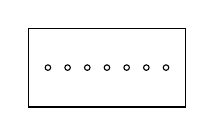
\begin{tikzpicture}
    \draw (0,0) rectangle (2,1);
    \foreach \x in {0.25,0.5,...,1.75} \draw (\x,0.5) circle (1pt);
  \end{tikzpicture}
  \caption{Simple TikZ demo.}
\end{figure}

If \texttt{pgfplots} is installed (we auto-load it if present), a quick plot:
\IfFileExists{pgfplots.sty}{%
\begin{figure}[h]
  \centering
  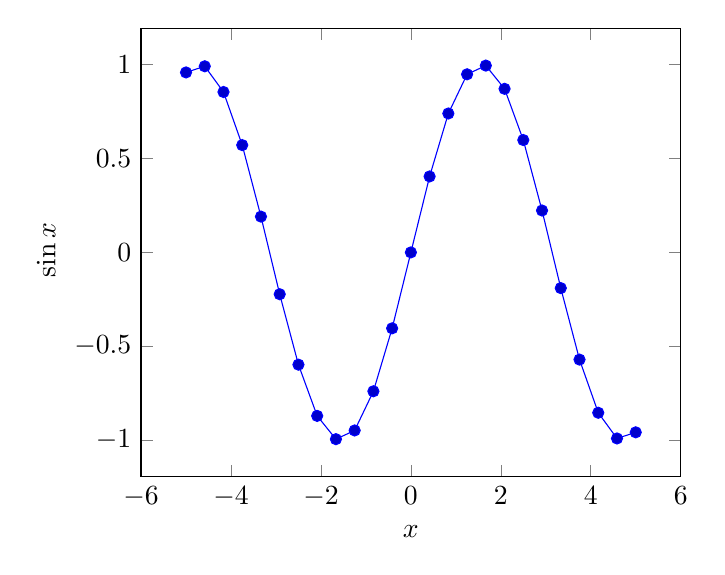
\begin{tikzpicture}
    \begin{axis}[xlabel=$x$,ylabel={$\,\sin x$}]
      \addplot {sin(deg(x))};
    \end{axis}
  \end{tikzpicture}
  \caption{Sine plot with pgfplots.}
\end{figure}
}{\noindent\emph{(pgfplots not installed — skipping plot.)}}

\section{Cross-references}
Use \verb|\label{...}| and \verb|\cref{...}| for equations, figures, tables, algorithms, and listings to get correct names and numbers automatically.

\section{Bibliography citation}
Cite like \cite{porter2008} and list all sources in the “Literature” section (managed by \texttt{biblatex} with the IEEE style in this project).

% ===== Declarations & Acknowledgments (if needed at end) =====
\frontmatterpage
\unchapter{Apliecinājums / Affirmation}
\textit{Ar šo es, \studentnameLV, apliecinu, ka bakalaura darbs ir izpildīts patstāvīgi, bez citu palīdzības, no svešiem avotiem ņemtie dati un definējumi ir uzrādīti darbā. Šis darbs nekādā veidā nav iesniegts nevienai citai pārbaudījuma komisijai un nekur nav publicēts.}

\vspace{12mm}
\noindent \textit{(Hereby I, \studentnameEN, affirm that the Bachelor's thesis was performed independently; sources of data and definitions are provided. This work has not been submitted to any other examination commission and has not been published elsewhere.)}

\vspace{14mm}
\noindent Rīga, 20\underline{\hspace{1cm}}.\ \underline{\hspace{2.5cm}}.\hspace{1cm}\rule{5cm}{0.4pt}\\
\hspace*{7.1cm}\scriptsize paraksts/signature, atšifrējums/decription \hfill

\frontmatterpage
\unchapter{Pateicības / Acknowledgments}
Autors izsaka pateicību darba vadītājam par sniegtajiem padomiem un atbalstu, kā arī uzņēmuma “X” kolēģiem par palīdzību datu iegūšanā un aptaujas realizēšanā.

The authors express gratitude to their supervisor for the provided advice and support, as well as to the colleagues at "X" company for their assistance in data acquisition and the implementation of the survey.

\end{document}
